\chapter{基于DTW距离度量的Shapelet并行算法设计}
\label{cha:chap04:myalg}

%本章首先~\ref{cha:chap04:myalg:Overview}介绍基于DTW距离度量的Shapelet并行算法总体流程、并行方案,整个流程主要按照定义~\ref{def:chap03:Threephases}的三个阶段来执行的:距离计算阶段(~\ref{cha:chap04:myalg:DTW},~\ref{cha:chap04:myalg:euclid})、最佳分割点计算阶段(~\ref{cha:chap04:myalg:infogain})、候选序列筛选阶段。

第三章主要介绍了基于DTW距离度量的Shapelet算法并行总体方案和流程以及一些并行前置技术。本章主要对于各并行模块的并行算法进行详细介绍,主要包括w>0距离计算阶段并行方案、w=0距离计算阶段并行方案、最佳分割点阶段并行方案。其中,候选序列筛选阶段因为主要是参考规约算法完成,可以参考文献~\cite{harris2007optimizing}中规约过程,在本章节中不做体现;CPU计算最佳分割点阶段采用和GPU计算最佳分割点采用相同的算法,在本章也不做叙述。
%第二章介绍了Shapelet的通用算法和基本定义,第三章介绍了GPU/CUDA并行原理、并行的难点,本章在前面介绍Shapelet和GPU/CUDA相关技术的基础上,提出了基于DTW距离度量的Shapelet并行算法。

\section{w>0距离计算阶段并行方案}
\label{cha:chap04:myalg:DTW}
本章主要介绍$w>0$时,距离计算阶段并行所使用的并行策略、并行算法设计、以及实现细节和性能考虑。在这一章讨论的都是基于$DTW(A,B,w)$距离讨论的。

\subsection{并行策略}

$w>0$距离计算阶段并行策略部分主要介绍$DTW(A,B,w)$如何使用“重用”策略降低算法时间复杂度和空间复杂度,以及如何被多线程并行利用。

首先,介绍一下如何使用重用策略降低算法时间复杂度。在章节~\ref{cha:chap02:generalalganalysis}提及,距离计算$Dist(A,B)$/$DTW(A,B,w)$是Shapelet算法中时间复杂度最高的操作,时间复杂度为$O(wN^2L^4)$。但是对于某个候选序列$S = T_{i,s}^{len}$,在进行距离计算阶段进行$\mathcal{F}$的计算,如公式~\ref{equ:chap04:dtwreuse},其中的最基本运算是$DTW(T_{i,s}^{len},T_{j,p}^{len},w)$。
%\begin{equation}
%\label{equ:chap04:dtwreuse}
%\mathcal{F}=\left\lbrace SubDist(S,T_j),j=1,2,\cdots,N\right\rbrace  =\left\lbrace \min_{p=1\to L-len+1}(DTW(T_{i,s}^{len},T_{j,p}^{len},w)),j=1,\cdots,N\right\rbrace 
%\end{equation}

%\begin{equation}
%\label{equ:chap04:dtwreuse}
%\begin{array}{l}
%\mathcal{F}=\left\lbrace SubDist(S,T_j),j=1,2,\cdots,N\right\rbrace \\ [0.3cm]
%=\left\lbrace \min_{p=1\to L-len+1}(DTW(T_{i,s}^{len},T_{j,p}^{len},w)),j=1,\cdots,N\right\rbrace 
%\end{array}
%\end{equation}
\begin{equation}
\label{equ:chap04:dtwreuse}
\begin{split}
\mathcal{F} &=\left\lbrace SubDist(S,T_j),j=1,2,\cdots,N\right\rbrace \\ 
&=\left\lbrace \min_{p=1\to L-len+1}(DTW(T_{i,s}^{len},T_{j,p}^{len},w)),j=1,\cdots,N\right\rbrace
\end{split}
\end{equation}

而对于整个Shapelet发现过程,即对于整个$SubSet(D)$中的所有候选序列$T_{i,s}^{len}$而言,公式~\ref{equ:chap04:BasicOp}是所有距离计算的集合,从公式中可以看出,数据集中任何两个长度相等的子序列$T_{i,s}^{len}$和$T_{j,p}^{len}$都会计算发生$DTW(A,B,w)$过程。%,长度为$len$的$DTW(A,B,w)$计算如公式~\ref{equ:chap04:BasicOp}。
%\begin{equation}
%\label{equ:chap04:BasicOp}
%DTW(T_{i,s}^{len},T_{j,p}^{len},w),i=1\to N,j=1\to N,s=1\to L-len+1,p=1\to L-len+1
%\end{equation}
%\begin{equation}
%\label{equ:chap04:BasicOp}
%\begin{array}{l}
%DTW(T_{i,s}^{len},T_{j,p}^{len},w),s.t.~i=1\to N,j=1\to N \\ [0.3cm]
%s=1\to L-len+1,p=1\to L-len+1 
%\end{array}
%\end{equation}
\begin{equation}\label{equ:chap04:BasicOp}
\left\{\begin{array}{l}
\left\lbrace DTW(T_{i,s}^{len},T_{j,p}^{len},w) \right\rbrace \\[0.1cm]
\mbox{subject to:}\\[0.1cm]
\qquad len = 1 \to L \\[0.1cm]
\qquad i=1\to N,j=1\to N\\[0.1cm]
\qquad s=1\to L-len+1,p=1\to L-len+1 
\end{array}\right.
\end{equation}



对于长度$len,len=1\to M$不同的$DTW(T_{i,s}^{len},T_{j,p}^{len},w)$计算有这大量的重复计算,这里使用$A_{1:len}=T_{i,s}^{len}$,$B_{1:len}=T_{j,p}^{len}$来代替$T_{i,s}^{len},T_{j,p}^{len}$讨论重复计算。如图~\ref{fig:DTWParallel}所示,在$DTW(A_{1:M},B_{1:M},w)$的动态计算过程中可以囊括M个距离计算$DTW(A_{1:m},B_{1:m},w),m=1,2,\cdots,M$。而在使用重用策略下,$DTW(A_{1:m+1},B_{1:m+1},w)$可以视为在$DTW(A_{1:m},B_{1:m},w)$的基础上完成,时间复杂度均摊到每一对距离计算$DTW(A_{1:m},B_{1:m},w)$为$O(w)$而不是$O(wL)$的时间复杂度。因为候选序列$S$计算$\mathcal{F}$的过程包含$O(NL)$个$DTW(T_{i,s}^{len},T_{j,p}^{len},w)$计算,单个候选序列$S$计算$\mathcal{F}$的均摊时间复杂度为$O(wNL)$。在数据集$D$所有候选序列集合$SubSet(D)$共有$O(NL^2)$个元素,因为使用重用策略时,基于DTW距离度量的Shapelet算法时间复杂度为$O(NL^2*wNL)=O(wN^2L^3)$。而原始基于DTW度量的Shapelet发现算法时间复杂度为$O(wN^2L^4)$,通过重用策略可以降低整个算法的时间复杂度,降低执行时间。算法~\ref{alg:originplus}是使用重用策略下基于DTW度量的Shapelet串行算法。
%同理,在基于DTW度量的Shapelet算法上,
%$SubDist(T_{i,s}^{L-s},T_j),j=1,2,\cdots,N$可以包含$SubDist(T_{i,s}^{len},T_j),len=1,2,\cdots,L-s,j=1,2,\cdots,N$,总的时间复杂度为$O(wNL^2)$,而每个候选序列$S=T_{i,s}^{len}$均摊时间复杂度。=
%假设$A_{1:M},B_{1:M}$是数据$D$中任意两个长度为$M$的子序列或候选序列,
%$S$和所有等长的时间子序列(候选序列)都进行了距离计算。也就是说,在Shapelet算法中,任何两个长度相等的子序列都会进行一次距离计算,距离计算之间存在着关系,在这些距离计算之间可以通过一些重用的策略避免每一个对距离计算都要花费$O(wL)$($DTW(A,B,w)$的时间复杂度)的时间。
%而在数据集$D$中,$T_{i,s},i=1,2,\cdots,N,s=1,2,\cdots,L$这样的元素候选序列有$O(NL)$个,而$SubDist(T_{i,s}^{L-s},T_j),j=1,2,\cdots,N$中包含$O(NL)$个$DTW(A,B,w)$计算,则Shapelet算法的时间复杂度为$O(NL*NL*wL)=O(wN^2L^3)$。
\begin{figure}[H] % use float package if you want it here
	\centering
	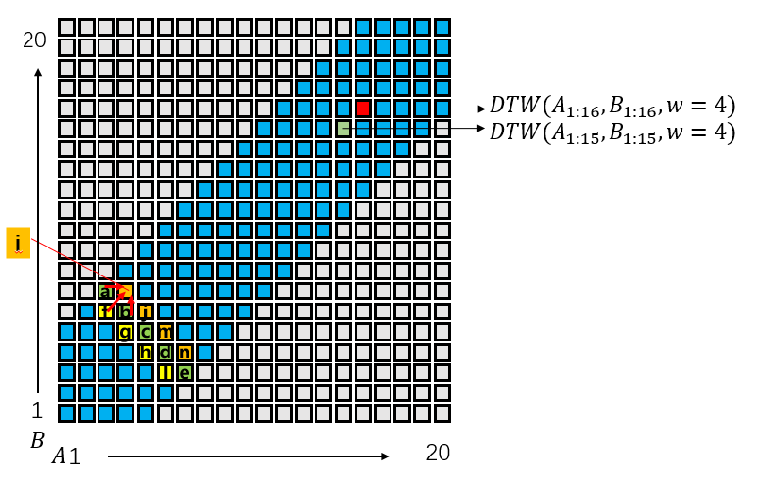
\includegraphics[height=8.2cm]{DTWParallel.png}
	\caption{“重用”降低时间空间复杂度和如何并行$DTW(A,B,w)$计算}
	\label{fig:DTWParallel}
\end{figure}
\begin{algorithm}
	\caption{基于DTW距离度量的Shapelet串行算法(使用重用策略之后)}
	\label{alg:originplus}
	\begin{algorithmic}[1]
		\Function{ShapeletAlg}{$D$}
		%\State $CENTER \gets (w+1)/2$;
			\State $lastS \gets \phi, lastinfogain \gets 0, lastdosp \gets 0, leftisAorB = A$
			\ForAll{$S \in \left\lbrace T_{i,s}^{L-s},i=1,2,\cdots,N,s=1,2,\cdots,L \right\rbrace $}
				%\State $\mathcal{F} = \left\lbrace (...,SubDist(S,T_j),y_j),...\right\rbrace,j = 1,2,\cdots,N$
				\For{$i = 1$ to $|S|$}
					\If{$1 = i$}
						\State 计算$SubDist(S_{1:1},T_j,j=1,2,\cdots,N)$获得$\mathcal{F}_{S(1:1)}$ \label{dtw1}
					\Else
						\State 在$\mathcal{F}_{S(1:i-1)}$的基础上计算$\mathcal{F}_{S(1:i)}$ \label{dtw16basedtw15}
					\EndIf
					\State 计算$g(D,(S,d_{osp(S(1:i))}))$
					\If{$g(D,(S,d_{osp(S(1:i))})) > lastinfogain$}
						\State 更新$lastinfogain$,$lastS$,$lastdosp$,$leftisAorB$
					\EndIf
				\EndFor
			\EndFor
			\State \Return $lastinfogain$,$lastS$,$lastdosp$,$leftisAorB$
		\EndFunction
	\end{algorithmic}
\end{algorithm}

并行过程能否顺利执行和DTW计算的空间复杂度有很大关系,因为在并行计算中,DTW计算需要占据共享内存空间。如何降低DTW计算的空间复杂度,$DTW(A_{1:m+1},B_{1:m+1},w)$都是依赖$DTW(A_{1:m},B_{1:m},w)$的计算结果而来的,而$DTW(A_{1:m+1},B_{1:m+1},w)$的计算和$DTW(A_{1:m},B_{1:m},w)$之前的代价矩阵元素没有关系,因此计算时只需要保留和$DTW(A_{1:m},B_{1:m},w)$之间的代价矩阵部分元素即可,如图~\ref{fig:DTWParallel}中并行依赖计算部分,因此空间复杂度为$O(w)$,这样可以大大减少共享内存的使用。

最后讨论一下如何使用多线程对于$DTW(A_{1:m+1},B_{1:m+1},w)$并行计算。如图~\ref{fig:DTWParallel},将从$DTW(A_{1:m+1},B_{1:m+1},w)$到$DTW(A_{1:m},B_{1:m},w)$之间计算过程提取出来,分别$even$和$odd$表示偶数和奇数对角线的元素,则原本代价矩阵中的递归方程将从$d_{x,y}=|a_x-b_y|_n + \min(d_{x,y},d_{x-1,y},d_{x,y-1})$变为公式~\ref{equ:chap04:dtwparallelequ}方程。
\begin{equation}
\label{equ:chap04:dtwparallelequ}
D_{x,y} = 
\begin{cases}
even_t=|a_x-b_y|_n+\min(even_t,odd_t,odd_{t+1}) & \text{if $x+y$ is even }\\
odd_{t+1}=|a_x-b_y|_n+\min(odd_{t+1},even_t,,even_{t+1}) & \text{if $x+y$ is odd}\\
\end{cases}
\end{equation}
这样就可以通过$even$和$odd$交替更新完成整个代价矩阵上的元素$D_{x,y}$的更新,而且可以通过多并行线程完成,至于$t$和$x,y$可以通过一定的对应方式计算,这里不做过多介绍。这里并行计算一个$DTW(A,B,w)$的线程个数为$w+1$的公约数$y,s.t. mod(w+1,y)=0$为宜,因为并行依赖区域的宽度最大为$w+1$,使用$y$个线程并行计算$D_{x,y}$可以保证多个线程的执行内容是均衡的,不会造成计算资源的浪费。

%的并行依赖计算部分是对于相邻的两个$DTW(A_{1:m},B_{1:m},w)$
%
%为了多线程可以配合计算一个
%在DTW测度距离$DTW(A_{1:M},B_{1:M},w)$过程中,涵盖了$M-1$个$DTW(A_{1:i},B_{1:i}),i=1,2,\cdots,M-1$距离结果,当每个$DTW(A_{1:i},B_{1:i}),i=1,2,\cdots,M$单独计算时,每个时间复杂度为$O(wM)$,总体时间复杂度为$O(wM^2)$;当$DTW(A_{1:i},B_{1:i}),i=1,2,\cdots,M$一起计算时,$DTW(A_{1:i+1},B_{1:i+1})$在$DTW(A_{1:i},B_{1:i})$的基础上计算,时间复杂度为$O(w)$,当使用这种增量的算法逐步计算所有DTW距离时,总的时间复杂度为$O(wM)$。
%
%$SubDist(S,T_j)$是在$O(L)$个距离值中取最低值,根据上面提到的增量计算,$SubDist(S_{1:i+1},T_j)$在$SubDist(S_{1:i},T_j)$基础上计算的时间复杂度为$O(wL)$。$\mathcal{F}$包含$N$个$SubDist(S_{1:i+1},T_j)$计算,其中$j=1,2,\cdots,N$,则$\mathcal{F}_{S(1:i+1)}$在$\mathcal{F}_{S(1:i)}$基础上计算时间复杂度为$O(wNL)$。

%{\color{red}{两个相互依赖的DTW计算中间的依赖空间复杂度是$O(w)$,可以参考一下算法~\ref{alg:originplus}}}


%{\color{red}{原始算法需要放在前面去}}

%在算法~\ref{alg:originplus}中,算法只计算集合$\left\lbrace T_{i,s}^{L-s},i=1,2,\cdots,N,s=1,2,\cdots,L \right\rbrace$中所有候选序列$S$和数据集$D$中所有时间序列$T_j$的距离$\mathcal{F}_{S}$,至于$\mathcal{F}_{S(1:i)},i=1,2,\cdots,|S|$都会在$\mathcal{F}_{S}$计算过程中产生。

%{\color{red}{空间复杂度这块是为了节省共享内存使用,可以放在技巧哪里和DTW并行计算一块进行}}
%$\mathcal{F} = SubDist(S,T_j),j=1,2,\cdots,N$计算只需要$Dist(A,B)$或$DTW(A,B,w)$的结果,并不需要知道$A,B$的如何进行对齐的,因此只要保留$O(2w)$的空间即可完成结果计算。
%关于$DTW(A,B,w)$的空间复杂度,$DTW(A_{1:i+1},B_{1:i+1})$都是基于$DTW(A_{1:i},B_{1:i})$基础计算的,只需要保留两者之间限制区域的元素即可,不需要其他空间,而且空间可以交替使用,因此在$DTW(A,B,w)$只需要保留$O(2w)$的空间即可,不需要$O(wL)$的空间复杂度。


\subsection{并行算法设计}

本章节主要根据伪码介绍一个Block的多个线程是如何运行的,其中$Block(i,s)$中线程$(tidx,~)$负责$T_i$中以$s$位置为起始的所有候选序列$T_{i,s}^{len},len=1\to L-s$和几个时间序列$T_j$的距离,如\ref{equ:chap04:everythread}。
%\begin{equation}
%\label{equ:chap04:everythread}
%SubDist(T_{i,s}^{len},T_j),len=1\to(L-s),j=\left\lbrace tid_x,tid_x+dim_{tidx},tid+2*dim_{tidx},\cdots \right\rbrace 
%\end{equation}
%\begin{equation}
%\label{equ:chap04:everythread}
%\begin{array}{l}
%SubDist(T_{i,s}^{len},T_j),s.t.~len=1\to(L-s), \\ [0.3cm]
%j=\left\lbrace tid_x,tid_x+dim_{tidx},tid+2*dim_{tidx},\cdots \right\rbrace 
%\end{array}
%\end{equation}
\begin{equation}\label{equ:chap04:everythread}
\left\{\begin{array}{l}
\left\lbrace SubDist(T_{i,s}^{len},T_j) \right\rbrace \\[0.1cm]
\mbox{subject to:}\\[0.1cm]
\qquad len=1\to (L-s)\\[0.1cm]
\qquad j=\left\lbrace tid_x,tid_x+dim_{tidx},tid+2*dim_{tidx}\right\rbrace 
\end{array}\right.
\end{equation}

算法~\ref{alg:kernel_ComputedtwsperblockForAll}是关于$Block(i,s)$中线程$(tidx,~)$运行过程,下面对于算法进行简单介绍:

\begin{breakablealgorithm}
	\caption{$Block(i,s)$中$(tid_x,tid_y)$线程计算$SubDist(T_{i,s}^{1\to (L-s)},T_j)$}
	\label{alg:kernel_ComputedtwsperblockForAll}
	\begin{algorithmic}[1]
		%\Require ~~\\
		%$T_{i,s}^{1 \to (L-s)}$: $T_i$中以$s$为起始的$L-s$个子序列\\
		%$(idx,len)$:GPU计算中的一个block,满足$idx < N,len < L$;\\
		%$T_j$:整个事件序列;\\
		%\Ensure ~~\\
		%$dist$:$T_{idx,s}^{len}$相对于每个时间序列的距离组成的数组
		\Function{kernel\_Computedtwsperblock}{$T_{i,s}^{1 \to (L-s)},T_j,w$}
		%\State $CENTER \gets (w+1)/2$;
			%\ForAll{$j \in thread_x$}
			\For{$j=tid_x;j \le N;t += dim_{tidx}$} \label{code:DTWCoalesced}
				%SubDist过程,比较L-s+1次
				\For{$p$ = $0$ to $L$} 
					\State $odd \gets \left\lbrace \infty\right\rbrace$,$even \gets \left\lbrace \infty\right\rbrace$,$even[center] \gets 0$
					\For{$step$ = $1$ to $longest$} \label{code:DTWParallel}
						%\State Calc the location of the most left-up point:$x_0,y_0$
						\State 计算$tid_y=0$线程的代价矩阵对应元素位置$x_0,y_0$
					%	\FOR{ $t=tid;t<w+1;t+=dim_{tid}$ } 
						%\For{$i$ = $tid$ to $2*w+2$}
						\For{$t=tid_y;t \le w+1;t += dim_{tidy}$} \label{code:dtwparallelequst}
							\State $x \gets x_0 + t, y \gets y_0 - t$
							\If{$x,y \in prunedtwZone$} \label{code:prunedtwZone}
								\State $even_t = (T_{j,x}-T_{i,y})^2 +\min(even_t,odd_t,odd_{t+1})$
							\EndIf
						\EndFor
						\State 将$even_{center}$和对应的$\mathcal{F}_j$比较求出最小值并更新$\mathcal{F}_j$ \label{code:dtwcompare0toL}
						%这里需要定义一个Dist(T_i^len,T_j);
						%\State Compare the $even[center]$($Dist(T_{idx,st}^{step},T_{j,u})$) with prior $Dist(T_{idx,st}^{step},T_j)$ and save the minimum.
						\State 计算$tid_y=0$线程的代价矩阵对应元素位置$x_0,y_0$
						%\State Calc the location of the most left-up point:$x_0,y_0$
						\For{$t=tid;t \le w+1;t += dim_{tid}$}
							\State $x \gets x_0 + t, y \gets y_0 - t$
							\If{$x,y \in prunedtwZone$}
								\State $odd_{t+1}=(T_{j,x}-T_{i,y})^2 +\min(odd_{t+1},even_t,,even_{t+1})$
							\EndIf
						\EndFor  \label{code:dtwparallelequed}
					\EndFor
				\EndFor
			\EndFor
		\EndFunction
	\end{algorithmic}
\end{breakablealgorithm}

1.$line$~\ref{code:DTWParallel}循环对应一个$DTW(T_{i,s}^{len},T_{j,p}^{len},w),len=1\to longest$计算过程;

2.$line$~\ref{code:dtwparallelequst}-\ref{code:dtwparallelequed}进行的是通过$dim_{tidy}$个线程完成一次DTW并行依赖计算,见图~\ref{fig:DTWParallel}并行依赖计算;

3.$line$~\ref{code:dtwcompare0toL}进行的$\min(DTW(S,T_{j,p}^{|S|},w)),p=1\to L-|S|+1$中的一次比较运算。

4.$line$~\ref{code:prunedtwZone}中的$prunedtwZone$表示代价矩阵限制区域,区域以外的不做更新。


\subsection{实现细节与性能考虑}
\label{cha:chap04:myalg:DTW:trick}
前两部分介绍了Shapelet并行策略和算法,这一部分就一些实现细节和性能考虑进行了阐述,主要从全局内存访问和存储体冲突两个角度进行介绍:

\begin{figure}[H] % use float package if you want it here
	\centering
	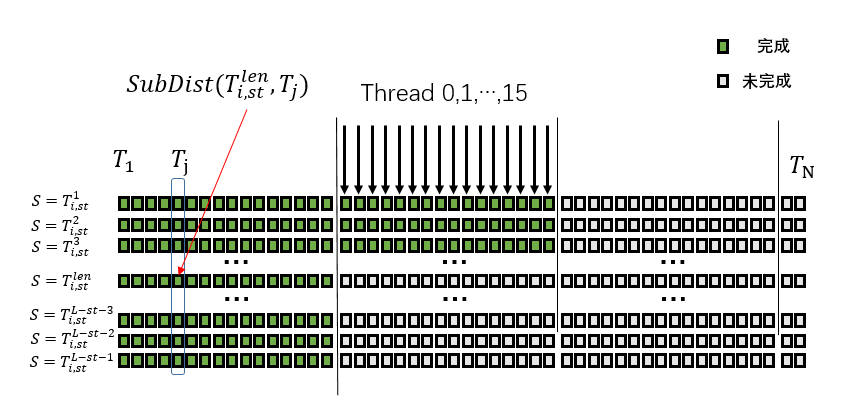
\includegraphics[height=7.2cm]{DTWglobalMem.png}
	\caption{$w>0$距离计算阶段中$\mathcal{F}$在全局内存中存储方式}
	\label{fig:DTWglobalMem}
\end{figure}

首先,介绍一下全局内存访问Coalesced和基于DTW度量的Shapelet算法结合。因为在算法~\ref{alg:kernel_ComputedtwsperblockForAll}中$line$~\ref{code:dtwcompare0toL}设计大量的全局内存访存过程,对于一个Block来说,需要经历$O(NL^2)$次访存,如果不做任何处理,会造成大量的等待延时,从而影响执行时间。

算法~\ref{alg:kernel_ComputedtwsperblockForAll}中$line$~\ref{code:dtwcompare0toL}并不是只有一个线程进行访存操作,而是有$dim_{tidx}$($line$~\ref{code:DTWCoalesced})个线程完成$DTW(T_{i,s}^{len},T_j),j=m*dim_{tidx}+1\to (m+1)*dim_{tidx}$一个过程,这$dim_{tidx}$个线程同时一段内存进行操作,这段内存是$T_{i,s}^{len}$对应的$\mathcal{F}$的$m*dim_{tidx}+1\to (m+1)*dim_{tidx}$位置,即$\mathcal{F}_{m*dim_{tidx}+1\to (m+1)*dim_{tidx}}$,当$dim_{tidx}=16,m=1$时,对应图~\ref{fig:DTWglobalMem}中红色部分。

合并内存访问的应用是如何进行的?如图~\ref{fig:DTWglobalMem},一个Block内的线程每循环一次,获得$\mathcal{F}_{16m+1\to16m+16}=SubDist(T_{i,s}^{len},T_j),j=16m+1,16m+2,\cdots,16m+16,m=0,1,2,\cdots$。$\mathcal{F}_{16m+1\to 16m+16}$在全局内存中是连续的地址空间,Block中的多个线程可以通过内存合并访问来提高全局内存访问效率。

然后介绍一下存储体冲突和算法结合使用,算法~\ref{alg:kernel_ComputedtwsperblockForAll}中的$even$和$odd$变量是使用共享内存存储的,$even$和$odd$与多线程配合完成$DTW(A,B,w)$的计算过程。$even$和$odd$在共享内存中占$2(w+2)$大小的共享内存,这样容易造成存储体冲突Bank-Conflict,最起码会产生2-Way Conflict现象,当$w=6$时出现16-way Conflict,使得线程访问存储体被大量序列化,使执行效率大大降低。

\begin{figure}[H] % use float package if you want it here
	\centering
	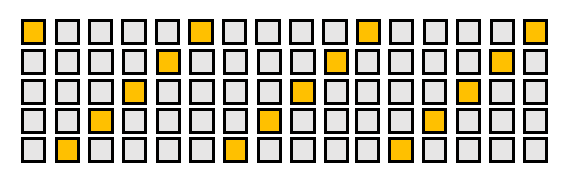
\includegraphics[height=4.5cm]{bankconflicteven.png}
	\caption{Stride选择与存储体冲突}
	\label{fig:BankConflictEven}
\end{figure}

这里将连续的两个线程的访问间隔$stride$设置为大于实际$2(w+2)$的最小奇数,即$stride=2w+5$,可以保证半个Warp内的所有线程可以访问到不同存储体,因为$stride$为奇数时,和偶数(16)没有公约数,在$stride*16$的地址范围内不可能出现在同一个存储体内,如图~\ref{fig:BankConflictEven},使用奇数$stride=5$,可以保证$(5m+n)\%16,m=0,1,2,\cdots,..,n < 5$可以分到16个存储体上。


\section{w=0距离计算阶段并行方案}
\label{cha:chap04:myalg:euclid}

当$w=0$时,DTW距离等价于欧氏距离,但是DTW距离相比欧氏距离多$O(L)$个比较操作和访存操作($L$为时间序列长度),因此使用$Euclid(A,B)$代替$DTW(A,B,w)$。本章主要介绍$w=0$距离计算阶段的并行策略、并行算法设计以及实现细节和性能考虑。

\subsection{并行策略}
\label{cha:chap04:myalg:euclid:Strategies}

如主流程图~\ref{fig:generalflow}所示,每个线程需要完成一个候选序列$S$对于数据集$D$中所有时间序列$T_j,j=1,2,\cdots,N$计算距离$SubDist(S,T_j),j=1,2,\cdots,N$获得$\mathcal{F}_S$。

当某个线程对应的候选序列$S$为$S=T_{i,s}^{len}$,这里就候选序列$T_{i,s}^{len}$和其中一个时间序列的$T_j$的距离$SubDist(T_{i,s}^{len},T_j)$进行分析。$SubDist(T_{i,s}^{len},T_j)$包含$O(L)$个欧氏距离$Euclid(T_{i,s}^{len},T_{j,p}^{len}),p=1,2,\cdots,L-len+1$的计算过程并在取其中的最小值,如图~\ref{fig:euclidparallel}中的线程s及其计算结果。其中欧式距离$Euclid(T_{i,s}^{len},T_{j,p}^{len})$欧式距离定义如公式~\ref{equ:chap04:eucliddef}:
\begin{equation}
\label{equ:chap04:eucliddef}
Euclid(T_{i,s}^{len},T_{j,p}^{len}) = \sum_{m=0}^{len-1}d(T_{i,s+m},T_{j,p+m})
\end{equation}
$Euclid(T_{i,s}^{len},T_{j,p}^{len})$的时间复杂度为$O(L)$。

另一线程的欧式距离$Euclid(T_{i,s+1}^{len},T_{j,p+1}^{len})$可以在$Euclid(T_{i,s}^{len},T_{j,p}^{len})$的基础上以$O(1)$的时间复杂度完成,如公式~\ref{equ:chap04:euclid}和图~\ref{fig:euclidparallel}黄框元素对红框元素的依赖。
\begin{equation}
\label{equ:chap04:euclid}
Euclid(T_{i,s+1}^{len},T_{j,p+1}^{len}) = Euclid(T_{i,s}^{len},T_{j,p}^{len}) + d(T_{i,s+len},T_{j,p+len}) - d(T_{i,s},T_{j,p})
\end{equation}

如图~\ref{fig:euclidparallel},所有的$Euclid(T_{i,s+1}^{len},T_{j,p+1}^{len})$在满足$s\geq1,p\geq1$的条件下都可以在$Euclid(T_{i,s}^{len},T_{j,p}^{len})$以$O(1)$的时间内通过线程之间的协作完成。但是$Euclid(T_{i,0}^{len},T_{j,p}^{len})$和$Euclid(T_{i,0}^{len},T_{j,0}^{len})$没有可以依赖的计算结果,只能通过原始定义~\ref{equ:chap04:eucliddef}。$Euclid(T_{i,0}^{len},T_{j,p}^{len}),q=1,2,\cdots,L-len$和$Euclid(T_{i,s}^{len},T_{j,0}^{len}),s=1,2,\cdots,L-len$共有$2(L-len)$个元素,均摊到每个线程有两个元素的计算量,时间复杂度为$O(L)$。

对于线程s来说,$SubDist(T_{i,s}^{len},T_j)$需要完成$L-len-1$次~\ref{equ:chap04:euclid}的依赖计算和2次~\ref{equ:chap04:eucliddef}次的原始计算,时间复杂度为$O(L)$。则线程s计算$SubDist(S,T_j),j=1,2,\cdots,N$获得$\mathcal{F}_S$时间复杂度为$O(NL)$,对于整个数据集的距离计算过程时间复杂度为$O(N^2L^3)$。

\begin{figure}[H] % use float package if you want it here
	\centering
	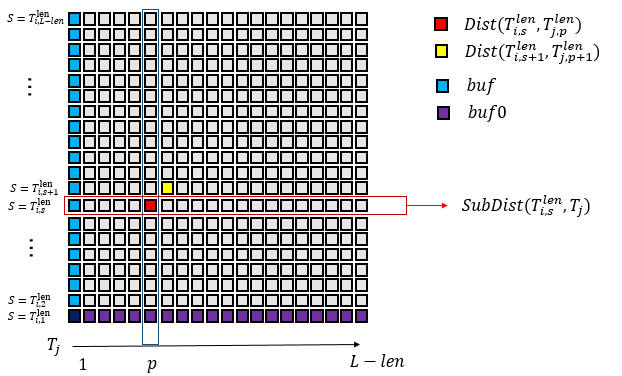
\includegraphics[height=8.2cm]{euclidparallel.png}
	\caption{$T_i$下长度为$len$的候选序列相对于$T_j$的距离计算($w=0$)}
	\label{fig:euclidparallel}
\end{figure}

\subsection{并行算法设计}
\label{cha:chap04:myalg:euclid:algdesign}

章节~\ref{cha:chap04:myalg:euclid:Strategies}介绍了$w=0$距离计算的并行原理,本章节将按照原理介绍算法设计部分。

\begin{breakablealgorithm}
	\caption{$Block(i,len)$中线程$s$计算$SubDist(T_{i,s}^{len},T_j),j=1,2,\cdots,L-len$}
	\label{alg:kernel_ComputeDist}
	\begin{algorithmic}[1]
		\Require ~~\\
		$T_{i,s}^{len}$:$block(i,len)$中线程$s$对应的候选序列,其中$(i,len)$作为距离计算grid一个block,满足$i \leq N,len \leq L$ \\
		$T_j$:整个时间序列
		\Ensure ~~\\
		$matrix$:矩阵,存储$Block(i,len)$下所有$S$对应的$\mathcal{F}$
		%$dist$:$T_{idx,s}^{len}$相对于每个时间序列的距离组成的数组
		%\Function{kernel\_ComputeDist}{$T_{i}$}
			\For{$j$ = $1$ to $N$}  \label{alg:kernel_ComputeDist:OutlineFor}
				\State $buf0[s]$ $\gets$ $0$ \label{alg:kernel_ComputeDist:eucliddefst}
				\State $buf[s]$ $\gets$ $0$
				\State $mindis[s] \gets 0$
				\For{$x$ = $1$ to $len$} 
					\State $buf0[s]$ $\gets$ $buf0[s]$ + $(T_{i,x}-T_{j,s+x})^2$  \label{alg:kernel_ComputeDist:dengjia1}
					\State $buf[s]$ $\gets$ $buf[s]$ + $(T_{i,s+x}-T_{j,x})^2$
				\EndFor  \label{alg:kernel_ComputeDist:eucliddefed}
				\State $maxdis[s] = buf[s]$	
				
				\For{$p$ = $1$ to $L-len+1$} \label{alg:kernel_ComputeDist:euclid}
					\If{$1 \neq s$}   \label{alg:kernel_ComputeDist:Warpdevergence1}
						\State $buf[s]$ $\gets$ $buf[s-1]$ + $(T_{i,s+len}-T_{j,p+len})^2$ - $(T_{i,s}-T_{j,p})^2$
					\EndIf
					\If{$1 = s$}     \label{alg:kernel_ComputeDist:Warpdevergence2}
						\State $buf[s]$ = $buf0[p]$ \label{alg:kernel_ComputeDist:dengjia2}
					\EndIf
					
					\State $maxdis[s]$ $\gets$ $min(maxdis[s],buf[s])$
				\EndFor
				\State Save $maxdis$ to the $jth$ lines of $matrix$ \label{maxdisoutput}
			\EndFor
			%\State \Return $dist$
		%\EndFunction
	\end{algorithmic}
\end{breakablealgorithm}

算法~\ref{alg:kernel_ComputeDist}是关于$w=0$距离计算的并行算法$Block(i,len)$中线程$s$的计算过程,下面关于算法进行介绍:

1.$line$~\ref{alg:kernel_ComputeDist:OutlineFor}的每一个循环对应的都是一个$SubDist(T_{i,s}^{len},T_j),j=1\to N$计算过程;

2.$line$~\ref{alg:kernel_ComputeDist:eucliddefst}-~\ref{alg:kernel_ComputeDist:eucliddefed}进行的两个欧式距离原始计算;

3.$line$~\ref{alg:kernel_ComputeDist:euclid}循环进行$L-len$次欧氏距离依赖计算。

4.$line$~\ref{maxdisoutput}是每个Block将众多$S$相对$T_j$的距离存储在$matrix$中的一行,$matrix$就是需要转置的矩阵。

\subsection{实现细节与性能考虑}
\label{cha:chap04:myalg:euclid:trick}

章节~\ref{cha:chap04:myalg:euclid:Strategies}和~\ref{cha:chap04:myalg:euclid:algdesign}分别介绍了$w=0$距离计算的并行原理和算法设计。本章从实现细节和性能考虑角度介绍$w=0$距离计算阶段,主要涉及到Warp分歧和矩阵转置在并行算法上的应用。

首先,$w=0$距离计算每个线程执行相同的内容并保持均衡。为了保持各线程之间均衡,原来需要在$line$~\ref{alg:kernel_ComputeDist:dengjia2}进行的$Euclid(T_{i,0}^{len},T_{j,p}^{len})$计算是放在了$line$~\ref{alg:kernel_ComputeDist:dengjia1}进行。如果不做这一项优化,线程0直接在$line$~\ref{alg:kernel_ComputeDist:dengjia2}处直接进行$Euclid(T_{i,0}^{len},T_{j,p}^{len})$计算,会使线程0在整个线程过程中执行$O(NL)$次欧式距离原始计算,使得线程0的时间复杂度为$O(NL^2)$,又因为Warp分歧的原因会使线程0所在的Warp所有线程都和线程0消耗相同的时间,因而$Block$执行时间成倍地增加执行时间,当一个Block中只有一个Warp的情况下,执行时间会增大32倍。

其次,$line$~\ref{alg:kernel_ComputeDist:Warpdevergence1}和$line$~\ref{alg:kernel_ComputeDist:Warpdevergence2}之间需要进行同步。因为$Euclid(T_{i,s}^{len},T_{j,p}^{len}),s=1,2,\cdots,L-len$和$Euclid(T_{i,s}^{len},T_{j,p+1}^{len}),s=1,2,\cdots,L-len$使用同一段共享内存$buf$,$Euclid(T_{i,s+1}^{len},T_{j,p+1}^{len})$都是在$Euclid(T_{i,s}^{len},T_{j,p}^{len})$基础上计算即$buf[s]$基于$buf[s-1]$计算,所以$buf[1]$的更新必须发生在$buf[s],s>1$更新之后。

最后主要介绍一下矩阵转置在算法上的应用,算法~\ref{alg:kernel_ComputeDist}的$line$~\ref{maxdisoutput}将多个候选序列相对于时间序列$T_j$的距离存在了对应矩阵$matrix$的第j行,如图~\ref{fig:euclidCoalescedSave}中$SubDist(S_m,T_j),m=1\to M$,则某个候选序列$S$对应的$\mathcal{F}$就存在于$matrix$中的某一列,如图~\ref{fig:euclidCoalescedSave}中$\mathcal{F}_{sm}$,$\mathcal{F}$对于最佳分割点阶段不是连续地址,这样不能直接进行最佳分割点计算。

实际上$\mathcal{F}$和$SubDist(S_m,T_j),m=1\to M$处于一个矩阵的行和列,不可能同时存在于连续地址中。为了解决不能同时进行连续地址访问的问题,我们在
$SubDist(S_m,T_j),m=1\to M$按行存储和$\mathcal{F}$按行读取之间添加了一个矩阵转置过程,如图~\ref{fig:euclidCoalescedSave}转化过程,这样就能保证$SubDist(S_m,T_j),m=1\to M$和$\mathcal{F}$都能进行连续地址的访问,从而保证了合并存储器的访问。而且矩阵转置有专门的算法可以使矩阵转置波特率达到全局内存之间数据拷贝的波特率~\cite{ruetsch2009optimizing}。

我们这里转置过程参考了CUDA矩阵转置算法~\cite{ruetsch2009optimizing},没有直接使用CUDA矩阵转置算法,主要基于两个原因:

一是每个block产生的矩阵大小不一样,主要是因为每个Block中线程个数不同,如果统一使用相同的矩阵转置算法会造成计算资源的浪费;

二是最佳分割点阶段要求$\mathcal{F}$之间是连续存储的,这就要求矩阵之间的存储不出现空白,但是按照CUDA矩阵转置算法调用会出现大量的空白,必须对转置之后的矩阵按行拼接起来,就需要在转置之后再增加一个拷贝调整过程,这样和我们优化效率的初衷不符。

\begin{figure}[H] % use float package if you want it here
	\centering
	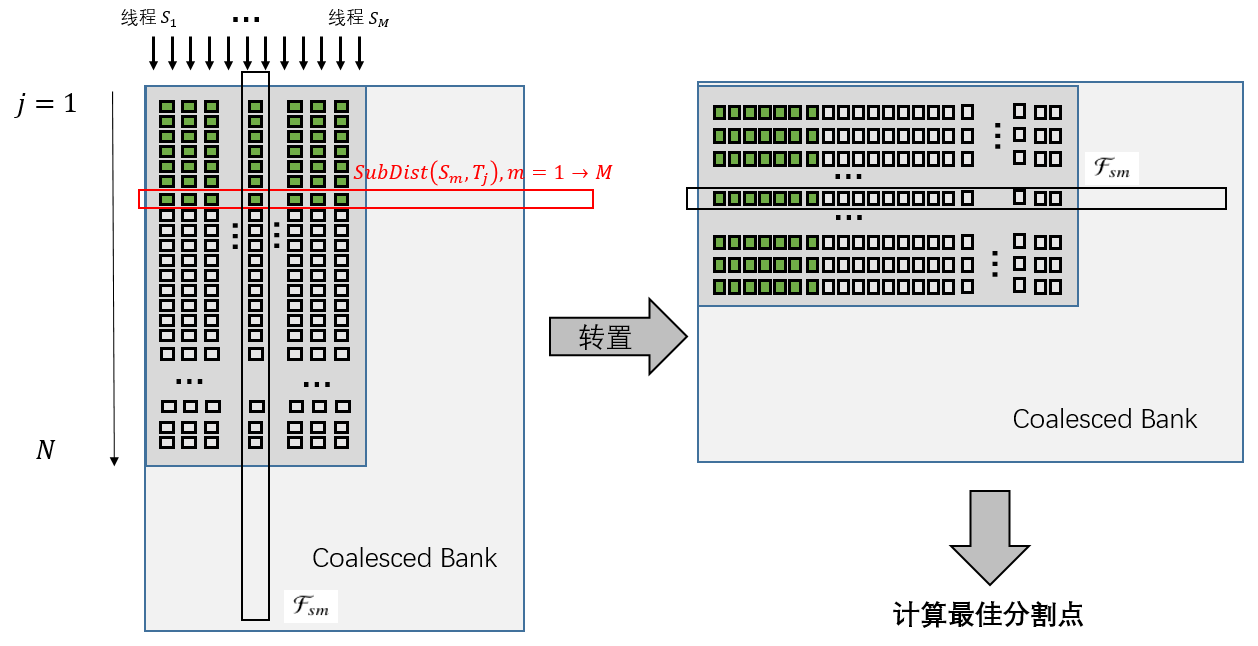
\includegraphics[height=8.2cm]{euclidCoalescedSave.png}
	\caption{矩阵转置同时满足距离计算阶段和最佳分割点计算阶段连续地址访问}
	\label{fig:euclidCoalescedSave}
\end{figure}

下面是我们如何对于以列形式存储的$\mathcal{F}$变成以行形式存储的方案,需要经过以下步骤:

1.首先在每个Block申请$M*33$的共享内存空间,如图~\ref{fig:transpose}的红字部分,Block将原来矩阵中的第一行$SubDist(S_m,T_1),m=1,\to M$读入共享内存的第一列(实际上是每33地址存一个元素),以此类推,直到存满32列共享内存;

2.Block其中一个Warp将共享内存中的第一行存入$S_1$对应$\mathcal{F}$的第一个128B空间,另一个Warp将第二行存入$S_2$对应$\mathcal{F}$的第一个128B空间,以此类推,对应图~\ref{fig:transpose}的Warp Coalesced过程;

3.$1,2$两步骤存入原始矩阵的前32行,按照这样每32行进行转置,从而完成整个过程的转置。

上面转置过程中,从全局内存中读入数据和向$\mathcal{F}$某个128B地址写入数据都是Coalesced过程,将共享内存设置成33列是为了避免出现存储体冲突,其中第33列元素不存储任何内容。

\begin{figure}[H] % use float package if you want it here
	\centering
	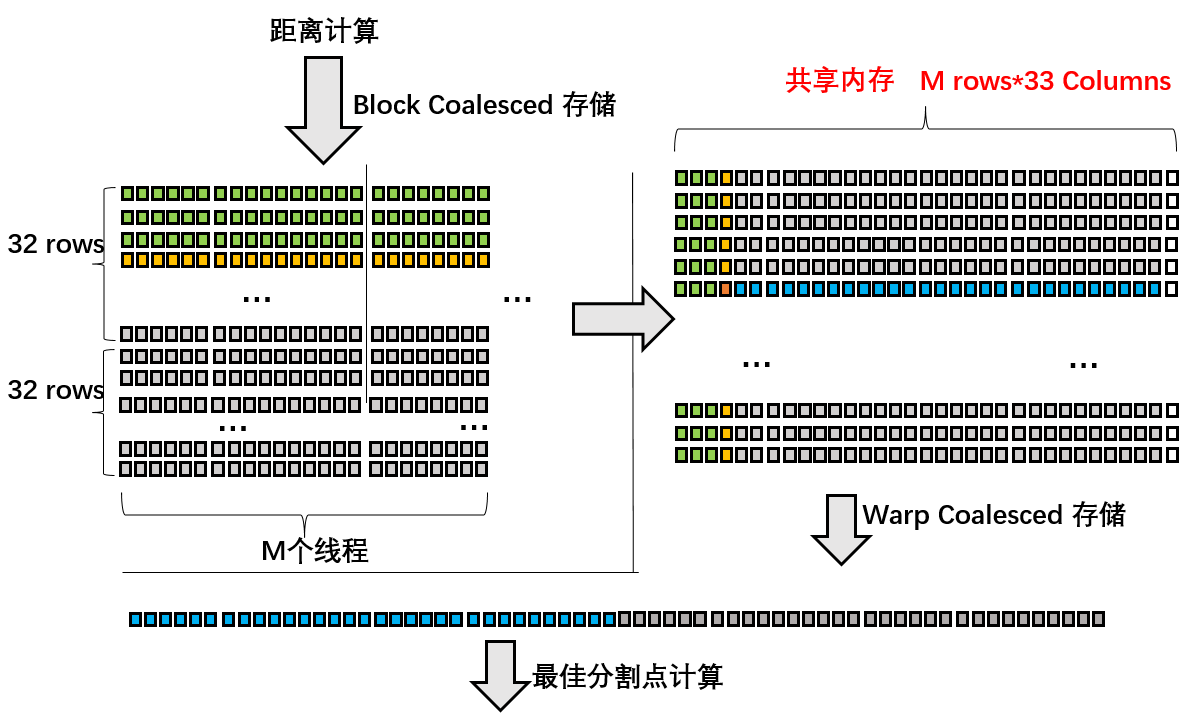
\includegraphics[height=9cm]{transpose.png}
	\caption{转置具体做法}
	\label{fig:transpose}
\end{figure}

相比基于$DTW(A,B,w=0)$的距离计算,本算法减少不必要的访存过程和比较过程,在执行时间性能上会表现的比较好。当然算法也是有缺陷的,时间序列长度$L$不能超过1024,因为线程之间需要通信才能完成依赖计算,GTX 1080一个Block中最多允许1024个线程,超过1024个线程的依赖关系不能建立。

\section{最佳分割点计算阶段并行方案}
\label{cha:chap04:myalg:infogain}

最佳分割点计算阶段是根据距离计算阶段的结果$\mathcal{F}$,求出一个分割点$d_{osp(S)}$使数据集$D$获得的信息增益$g(D,(S,d_{osp(S)}))$最大。

算法~\ref{alg:OriginInfogain}为计算最佳分割点的原始算法,其中$line$~\ref{code:sort}是对于$\mathcal{F}$排序,时间复杂度为$O(N\log(N))$。Line~\ref{code:maxinfogain}循环是以步进的方式计算获得的最大信息增益以及对应的分割点,时间复杂度为$O(N)$。因此从候选序列$S$对应的$\mathcal{F}$到计算最佳分割点复杂度为$O(N\log(N))$,但是对于整个候选序列集合$SubSet(D)$,时间复杂度度为$O(N^2L^2\log(N))$。

\begin{algorithm}
	\caption{最佳分割点计算原始算法}
	\label{alg:OriginInfogain}
	\begin{algorithmic}[1]
		\Function {CalcOptimalDividePoint}{$dist,label,N$}
			\State \Call{SortByKey}{$dist,label,key=dist$} \label{code:sort}
			%\State 计算最大信息增益/最佳分割点 \label{code:maxinfogain}
			\State $g(D,(S,d_{th}))\gets 0,dividepoint\gets 0.0,leftisAOrB\gets a$
			\For{$i=0$ to $N-1$} \label{code:} \label{code:maxinfogain}
				\State 计算$lefta,leftb,righta,rightb$ //$O(1)$%//以$\frac{dist[i]+dist[i+1]}{2}$为分割点,前面a个数,前面b个数,后面a个数,后面b个数.可以通过步进的方法在$O(1)$时间复杂度内完成.
				\State 根据$lefta,leftb,righta,rightb$计算信息增益$temp$ //$O(1)$
				\If{$temp > g(D,(S,d_{th}))$} //$O(1)$
					\State 更新$g(D,(S,d_{th})),dividepoint,leftisAOrB$
				\EndIf
			\EndFor
			\State \Return $g(D,(S,d_{th})),dividepoint,leftisAOrB$
		\EndFunction
	\end{algorithmic}
\end{algorithm}

最佳分割点总的时间复杂度为$O(N^2L^2\log(N))$,仅次于距离计算阶段的$O(N^2L^3)$(使用重用策略之后)。当数据集的大小$N$增大时,最佳分割点占比越高,从而影响整体执行时间。

\subsection{启发式算法设计}
\label{cha:chap04:myalg:infogain:design}

我们需要设计一个算法将最佳分割点计算的时间复杂度从$O(N\log(N))$降到$O(N)$,在这里,我们使用一种启发式计算分割点的算法来搜索最佳分割点。

图~\ref{fig:distancedistribute}为子序列$S$相对于数据集$D$中时间序列的距离-类标的集合$\mathcal{F}$,其中,横轴表示时间序列在数据集中的位置$j$,纵轴表示$S$与$j$位置时间序列$T_j$之间的距离$SubDist(S,T_j)$,颜色表示$T_j$的类标(A/B)。
\begin{figure}[H] % use float package if you want it here
	\centering
	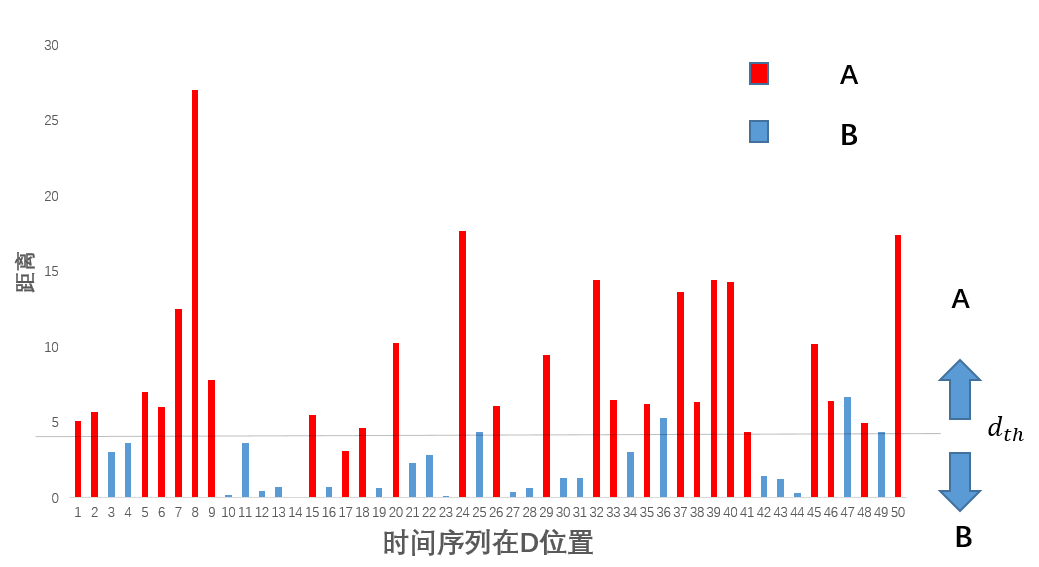
\includegraphics[height=6.2cm]{distancedistribute.png}
	\caption{$S$对于数据集$D$中时间序列的距离-类标集合,$\mathcal{F}$}
	\label{fig:distancedistribute}
\end{figure}

最佳分割点计算的目的在于寻找一个距离阈值$d_{th}=d_{osp(S)}$使得数据集$D$获得的信息增益$g(D,(S,d_{th}))$尽可能大,如图~\ref{fig:distancedistribute},满足$g(D,(S,d_{osp(S)}))>g(D,(S,d_{th})),\forall d_{th}\in \mathbb{R}_+$,并不是对于数据集按照距离$SubDist(S,T_j)$进行排序。算法~\ref{alg:OriginInfogain}是对于所有可能产生的信息增益$g(D,(S,d_{th}))$取值都进行了计算,相当于获得了一个全局最优值。

相比计算全局最优值,这里提供一种启发式的最优值搜索方式,二分地搜索到一个阈值,使得信息增益最大。首先介绍一下二分搜索地评价指标,根据公式~\ref{equ:chap2:Infogain2}可知,信息增益$g(D,(S,d_{th}))$最大化等价于条件熵$H(D|(S,d_{th}))$最小化\footnote{条件熵$H(D|(S,d_{th}))$恒大于$0$}。
存在一个点$d_{th}$将数据集$D$分为两个子集$D_1 = \left\lbrace T,SubDist(S,T)<d_{th} \& T\in D\right\rbrace $和$D_2 = \left\lbrace T,SubDist(S,T) \geq d_{th}\& T\in D\right\rbrace$,则条件熵$H(D|(S,d_{th}))$表达式如公式~\ref{equ:chap4:ConditionalEntropy},
\begin{equation}
\label{equ:chap4:ConditionalEntropy}
H(D|(S,d_{th})) = \frac{|D_1|}{|D|}H(D_1)+\frac{|D_2|}{|D|}H(D_2) = f(D_1) + f(D_2)
\end{equation}
为了方便叙述,这里将$\frac{|D_m|}{|D|}H(D_m),m=1,2$定义为$f(D_m),m=1,2$(对于数据集$D$而言,$|D|$为常数)。

假设在区间$(0,\infty)$一个分割点$d_{th1}$,将数据集$D$分为$D_1$和$D_2$。如果$f(D_1)>f(D_2)$,表示$D_1$的熵更高一点,可能在区间$(0,d_{th1})$存在一个阈值$d_{th2}$,使得条件熵$H(D|(S,d_{th_2}))$更低一些。这里对于$D$重新进行分割,将临近$D_1$在$(d_{th2},d_{th1})$地元素归入$D_2$数据集内,可能使$f(D_1)+f(D_2)$更小;反之,$(d_{th1},\infty$向相反方向寻找阈值,不断循环下去,呈现一个二分的搜索路线,直到分割点的搜索区间为空$0$为止。

上文每个区间都对应一个集合,比如$(0,\infty)$表示数据集$D$对应的所有$\mathcal{F}_j,j=1\to N$,在实际算法实现上没有使用区间的概念而是使用区间对应的集合$\left\lbrace \mathcal{F}_j,j=left\to right\right\rbrace $来进行二分搜索,当区间为0,即集合为$\phi$。

在任何一个区间对应的集合中可能存在不止一个元素,我们需要选择一个点作为阈值来对$D$进行切割,这里按照快排的思路和局部性的考虑选用集合最后一个元素(集合初始是无序的,最后一个元素不一定是最大或者最小)作为集合切割的阈值。 

算法~\ref{alg:HeuristicSplitInfogain}是启发式求最佳分割点算法:

算法中$dist$中表示候选序列$S$对数据集$D$时间序列的距离数组,即$\mathcal{F}$对应距离部分,$label$表示时间序列对应的类标。

$line$~\ref{alg:Heuristic:initial}为区间初始化,等价于搜索区间$(0,\infty)$;

$line$~\ref{alg:Heuristic:partion}是按照区间最后一个元素为切割点进行切割,详见算法~\ref{alg:HeuristicSplitInfogainBase};

$line$~\ref{alg:Heuristic:beforecalcentropy}-~\ref{alg:Heuristic:aftercalcentropy}为计算$f(D_1)$和$f(D_2)$并在$line$~\ref{alg:Heuristic:compare}比较并缩小搜索区间,可以在$O(1)$时间复杂度内完成;

$line$~\ref{alg:Heuristic:stop}表示如果连续两次条件熵呈增大趋势则返回上一次的分割点和条件熵。

\begin{breakablealgorithm}
	\caption{启发式算法计算最佳分割点算法$HeuristicOptimalSplitPoint$}
	\label{alg:HeuristicSplitInfogain}
	\begin{algorithmic}[1]
%	\Requre $dist,label$
%	\Ensure $lastEntropy,OptimalSplitPoint,leftisAOrB$
		\Function {HeuristicOptimalSplitPoint}{$dist,label,N$}
			\State $left \gets 1,right \gets N$  \label{alg:Heuristic:initial}
			\While{$left < right$}
				\State $p \gets $ \Call{Partion}{$dist, label, left, right$}  \label{alg:Heuristic:partion}
				%\State $lefta2 \gets $ \Call{Count\_if}{$label,left,p,0$}
				\State $lefta \gets \sum_{i\in BEFORE(p)}(label_i\in A)$ \label{alg:Heuristic:beforecalcentropy}
				\State $leftb \gets \sum_{i\in BEFORE(p)}(label_i\in B)$
				\State $righta \gets  \sum_{i \in BEHIND(p)}(label_i \in A)$
				\State $rightb \gets  \sum_{i \in BEHIND(p)}(label_i \in B)$
				%\State $pgoleftentropy \gets$
				\State $leftentropy \gets $ \Call{Entropy}{$lefta,leftb$}
				\State $rightentropy \gets $ \Call{Entropy}{$righta,rightb$} \label{alg:Heuristic:aftercalcentropy}
				\If{$leftentropy < rightentropy$}  \label{alg:Heuristic:compare}
				%\State $lefta1,leftb2 \gets lefta1 + lefta2,leftb1+leftb2$
				%\State 
					\State $left \gets p+1$
				\Else
				%\State $righta1,righta2 \gets righta1 + righta2,rightb1+rightb2$
					\State $right \gets p-1$
				\EndIf
				
				\If{$lastEntropy$ < $thisEntropy$}  \label{alg:Heuristic:stop}
					\State \Return $lastEntropy$以及对应分割点
				\EndIf
			\EndWhile
			\State \Return $thisEntropy$以及对应分割点
		\EndFunction
	\end{algorithmic}
\end{breakablealgorithm}

算法~\ref{alg:HeuristicSplitInfogain}可以看出,启发式是使用一种搜索的方式获得最佳分割点,我们可以把这个搜索分割点的过程称为最佳分割点搜索路线。

算法~\ref{alg:HeuristicSplitInfogainBase}是启发式计算最佳分割点中需要调用的算法,负责数据集$D$切割成$D_1,D_2$的函数$PARTION$.%,计算熵$ENTROPY$,条件熵$ENTROPYSPLIT$。
\begin{algorithm}
	\caption{最佳分割点计算的调用算法}
	\label{alg:HeuristicSplitInfogainBase}
	\begin{algorithmic}[1]
%		\Require $dist$数组,$label$数组
%		\Ensure $infogain$,$dividepoint$,$leftis$
		\Function {partion}{$dist, label, left, right$}
			\State $pivot$ $\gets$ $dist[right]$
			\State $p$ $\gets$ $left$
			\For{$q$ = $left$ to $right$}
				\If{$dist[q] < pivot$}
					\State \Call{swap}{$dist,p,q$}
					\State \Call{swap}{$label,p,q$}
					\State $p$ ++
				\EndIf
			\EndFor
			\State \Call{swap}{$dist,p,right$}
			\State \Return $p$
		\EndFunction
	\end{algorithmic}
\end{algorithm}

\subsection{随机排列shffule及其作用}
\label{cha:chap04:myalg:infogain:shuffle}

章节~\ref{cha:chap02:def}提及Shapelet的定义和本质,存在一种模式,数据集中一种时间序列$(label \in A)$和这种模式表现出较小的距离,另外一种$(label \in B)$则表现出较大的距离,Shapelet的本质是寻找这种模式。反之可以认为,与这种模式表现出较小距离的时间序列都存在能够表达这种模式的子序列,并且能够表达这种模式的候选序列不止一个。

能够表达这种特定模式的候选序列对于数据集中各时间序列表现出相似的距离度量。如图~\ref{fig:similardistance},$S1$、$S2$是两个能够区分两类时间序列的候选序列,两者相对于数据集中各时间序列表现的距离很接近。如果使用上述启发式算法,最佳分割点的搜索路线有可能是一致的,最后导致的分类效果是一样的。

\begin{figure}[H] % use float package if you want it here
	\centering
	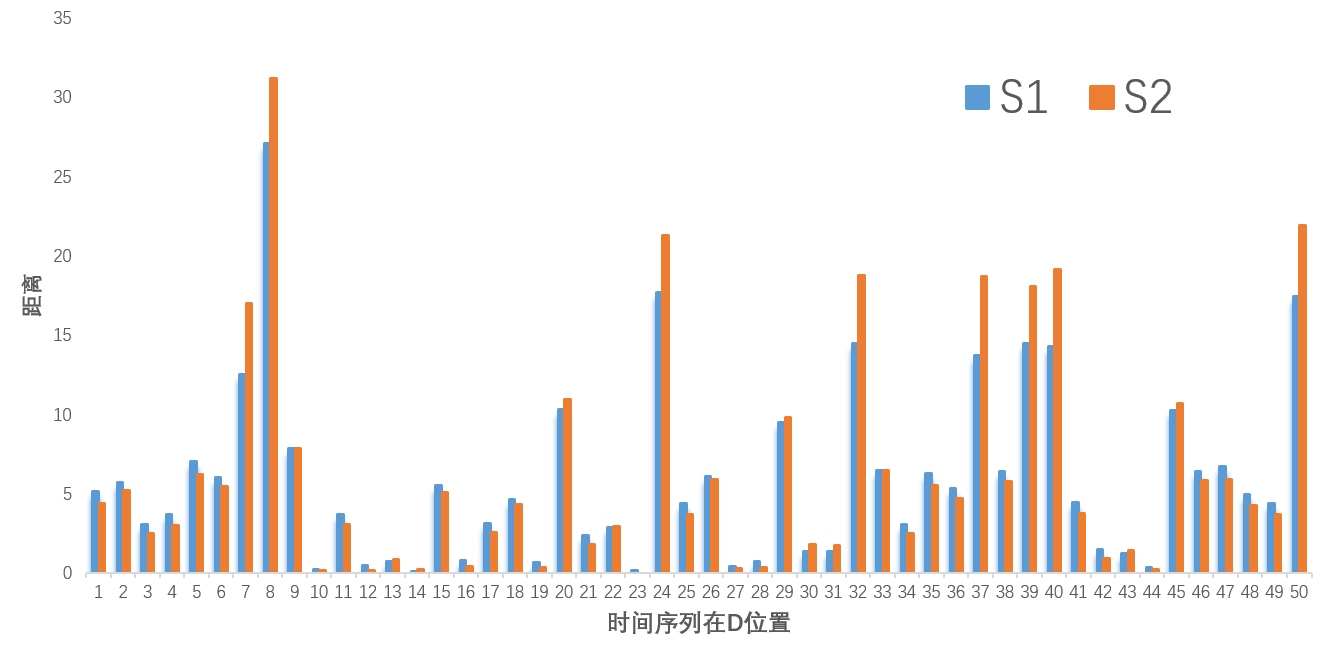
\includegraphics[height=7cm]{similardistance.png}
	\caption{$S1,S2$对于数据集$D$中时间序列距离的相似性}
	\label{fig:similardistance}
\end{figure}

启发式算法寻找的不是全局最优值,并不能保证这种唯一的搜索路线就能找最佳分割点。我们需要利用多个候选序列能够表达这种模式这一特点,使多个候选序列对应的启发式算法尽可能选择不同的最佳分割点搜索路线,目的是多个搜索路线中有某种搜索路线获得的结果和全局最优最接近。如何获得不同最佳分割点搜索路线,关键在于使用哪个点进行算法~\ref{alg:HeuristicSplitInfogainBase}的$patition$,启发式算法使用集合最后一个元素进行分割,而我们需要局部集合的最后一个元素不是同一个元素来使搜索路线不同,因此在计算最佳分割点之前需要对于$\mathcal{F}$进行随机排列Shuffle。

为了获得不同的最佳分割点搜索方式,在进行启发式算法搜索最佳分割点之前,对于$\mathcal{F}$进行随机排列Shuffle。算法~\ref{alg:ReservoirShuffle}是随机排列算法伪码,本文选择Kunth shuffle算法(可以使每个元素以$1/N$的概率出现在每个位置)进行随机排列,至于算法的选择原因在章节~\ref{cha:chap04:Heuristic:Skill}中结合GPU的使用介绍。

\begin{algorithm}
	\caption{对于$dist$和对应的$label$进行shuffle,$ReservoirShuffle()$}
	\label{alg:ReservoirShuffle}
	\begin{algorithmic}[1]
		\Require ~~\\
		$dist$ :候选序列$S$对数据集$D$时间序列的距离数组\\
		$label$:时间序列对应的类标\\
		$rng$ : 一个线程对应的随机数发生器
		\Ensure ~~\\
		$dist$:shuffle之后的$dist$\\
		$label$:shuffle之后的$label$
		\Function {ReservoirShuffle}{$dist, label, N, rng$}
			\For{$i$ = $2$ to $N$}
				\State $j$ $\gets$ $rng.$\Call{random}{$1,i$}
				\If{$i \neq j$}
					\State \Call{swap}{$dist,i,j$}
					\State \Call{swap}{$label,i,j$}
				\EndIf
			\EndFor
			\State \Return $dist$,$label$
		\EndFunction
	\end{algorithmic}
\end{algorithm}

\subsection{实现细节与性能考虑}
\label{cha:chap04:Heuristic:Skill}

章节~\ref{cha:chap04:myalg:infogain:design}和章节~\ref{cha:chap04:myalg:infogain:shuffle}讲述了启发式计算最佳分割点的过程,本章就算法的并行实现细节和性能考虑予以介绍。

章节~\ref{cha:chap04:myalg:infogain:shuffle}提及了Shuffle的选择吗,有多个可以选择的方案:Warp并行随机排列算法、调用Shuffle device函数、自实现随机排列函数。其中,Warp并行随机排列算法~\cite{nvidia2015c}虽然可以快速的实现一个随机排列算法,但是要求一个Warp内所有shuffle结果必须是一致的,不符合章节~\ref{cha:chap04:myalg:infogain:shuffle}使用shuffle的原因。调用现成的Shuffle device函数产生一个随机排列Index,对于每个线程需要占用$O(N)$的空间需要较多的GPU硬件资源。这里我们选择实现Kunth shuffle算法,可以在$O(N)$的时间复杂度下,以$O(1)$的额外空间复杂度完成随机排列Shuffle,算法按照蓄水池算法的原理,可以使每个元素出现在每个位置的概率为$O(1/N)$。

算法~\ref{alg:ReservoirShuffle}需要为每个线程提供不同的随机数发生器$rng$,否则,不同线程中使用相同的$rng$,最后导致随机数生成的过程是一致,Shuffle之后的结果依然是一致的。每个线程的随机发生器$rng$需要在进行启发式算法之前随机初始化,并且使用线程ID作为随机发生器的初始化参数之一。

最佳分割点计算阶段读入$\mathcal{F}$的方法:因为$\mathcal{F}$中的距离在距离阶段存储在连续空间中,每个线程读取一个$\mathcal{F}$的距离;$label$是通过合并内存访问读取到共享内存中。



\section{本章小结}

本章主要介绍总体方案设计中三处并行算法设计:w>0距离计算阶段并行方案,w=0距离计算阶段并行方案,最佳分割点计算阶段并行方案。
w>0距离计算阶段中每个线程负责一系列候选序列和几个时间序列之间的并行距离计算,并且使用全局内存访问和存储体冲突等技术和并行算法结合,加速了并行算法的执行。
w=0距离计算阶段通过线程之间协作完成了多个候选序列对于整个数据集中的时间序列并行计算距离,并且通过特定的矩阵转置方法使w=0距离计算阶段和最佳分割点阶段都可以同时进行连续地址访问,大大减少全局内存访存延时。
最佳分割点计算阶段使用了启发式计算最佳分割点和随机排列的方法完成了最佳分割点的并行计算,两者的结合保证了能够在准确率不降的前提下降低最佳分割点计算的执行时间。

%首先对于算法的整体流程和并行方案进行了概括介绍;然后对于距离计算阶段分别介绍针对和、算法设计以及并行实现细节和性能考虑;最后介绍了启发式计算最佳分割点的算法设计、Shuffle的使用及作用、并行实现细节和性能考虑。


